\documentclass[a0,landscape]{a0poster}
\usepackage{times}
\usepackage{graphicx}
\usepackage{geometry}
\usepackage{qrcode}
\usepackage{amssymb}
\usepackage[most]{tcolorbox}
\usepackage{alltt}

% --- Page Geometry (48x36 inches) ---
\geometry{papersize={48in,36in}, margin=1.2in}

% --- Custom Box Style ---
\newtcolorbox{posterbox}[1]{
    colback      = blue!5!white,
    colframe     = blue!75!black,
    fonttitle    = \bfseries\huge,
    title        = {#1},
    breakable,
    boxsep       = 6mm,
    arc          = 5mm,
}

\begin{document}
\pagestyle{empty}

% === TITLE BLOCK ===
\begin{center}
    \veryHuge \textbf{A Software Tool for Planning Better Clinical Trials} \\
    \vspace{0.25cm}
    \rule{\linewidth}{1.5pt}
    \vspace{0.25cm}
    \Huge \textbf{Arnab Aich} \hspace{1cm} Mentor: \textbf{Yuan Zhang}\\
    \huge \textit{Department of Preventive Medicine, University of Tennessee Health Science Center}
\end{center}
\vspace{0.5cm}

% === FLEXIBLE 3-COLUMN LAYOUT ===
\begin{minipage}[t]{0.32\linewidth} % --- LEFT COLUMN ---

\begin{posterbox}{The Challenge \& A Better Metric}
    \subsection*{\Large The Challenge of Trial Design}
    \large 
    Researchers must answer two key questions for an ethical and cost-effective study.
    \begin{enumerate}
        \item How many patients do we need? (Sample Size)  and 
        \item What accuracy can be achieved for a given cohort? (Power).
    \end{enumerate}

    \large
    In survival studies, we then follow the individuals over time to measure a \textbf{time-to-event} endpoint.
    

    \subsection*{\Large Why Traditional Methods Can Be Problematic}
    \large 
    Traditional metrics like the \textbf{Hazard Ratio (HR)} rely on strong assumptions that are often violated in the real world, making results hard to interpret.

    \vspace{0.25cm}\hrule\vspace{0.25cm}
    
    \subsection*{\Large A Better Metric: RMST}
    \large 
    % --- CORRECTED BOLD FONT ---
    We use \textbf{RMST} (Restricted Mean Survival Time). It directly measures the average "event-free" time.
    \begin{itemize} \itemsep=0.25em
        \item[\Large\checkmark]  It's easy for everyone to understand.
        \item[\Large\checkmark]  It provides a clear measure of treatment benefit.
    \end{itemize}
    \begin{center}
        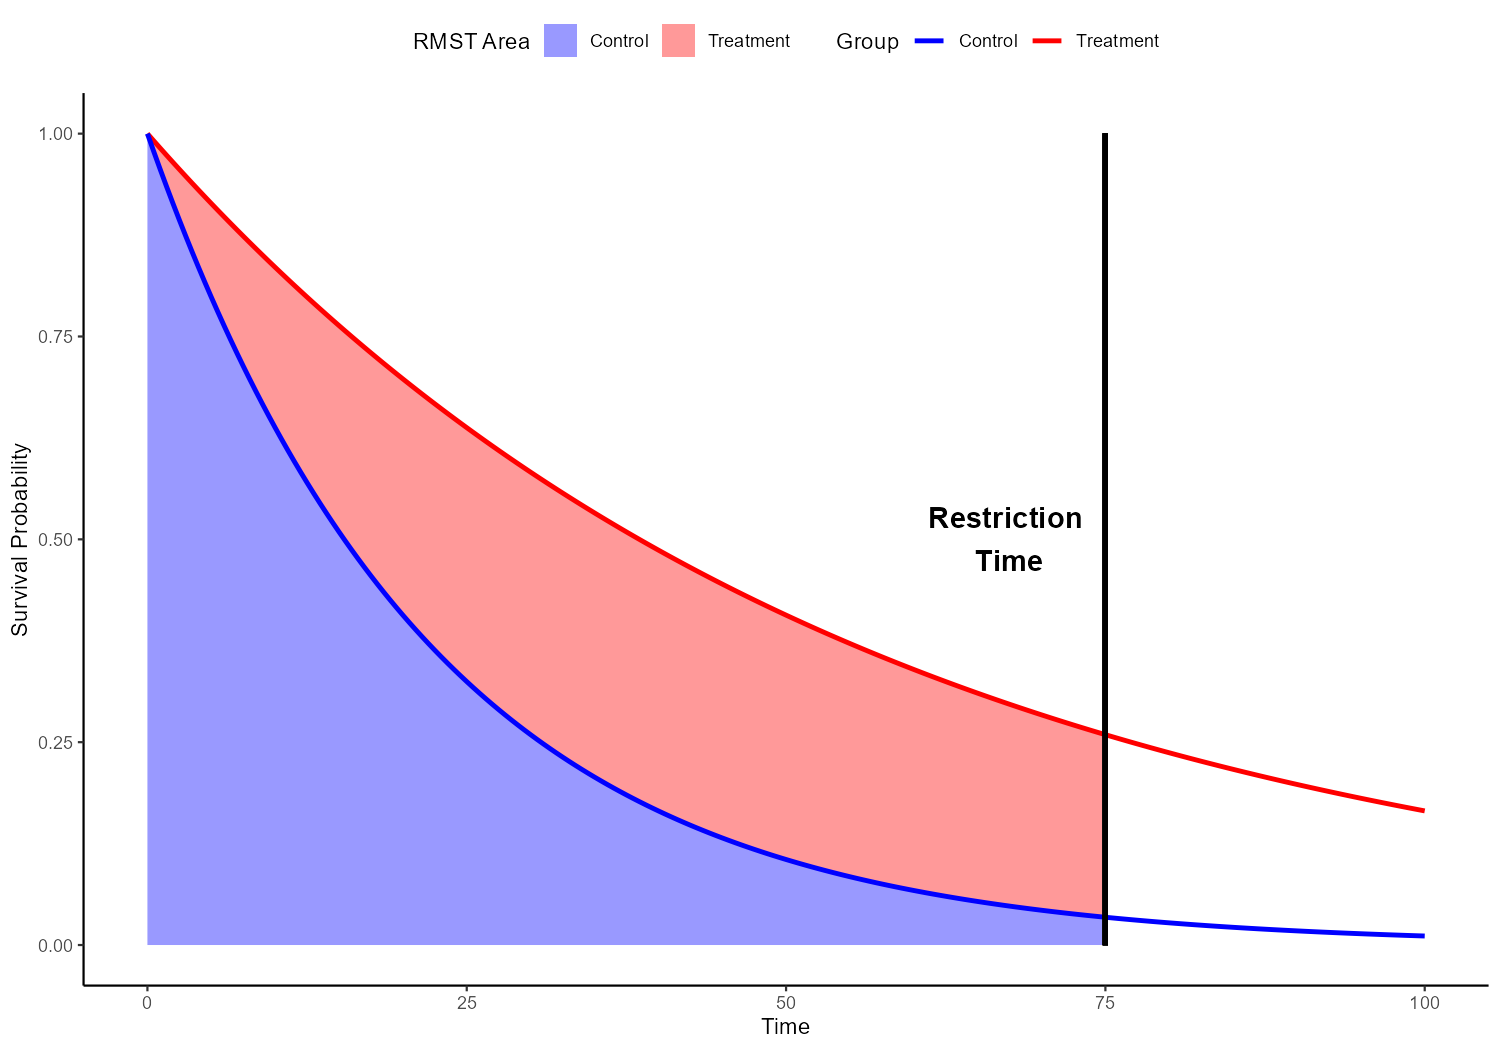
\includegraphics[width=\linewidth]{rmst_causal_plot.png}
    \end{center}
\large 
RMST difference provides causal interpretation which hazard ratios failed to provide.
\end{posterbox}

\end{minipage}
\hfill % Flexible space between columns
\begin{minipage}[t]{0.34\linewidth} % --- CENTER COLUMN ---

\begin{posterbox}{Our Solution: The `RMSTSS` Tool}
    \large
    Planning studies with RMST has been difficult. We made it easy. `RMSTSS` is a free tool that helps researchers properly plan modern medical studies.
    \begin{center}
        \vspace{0.25cm}
        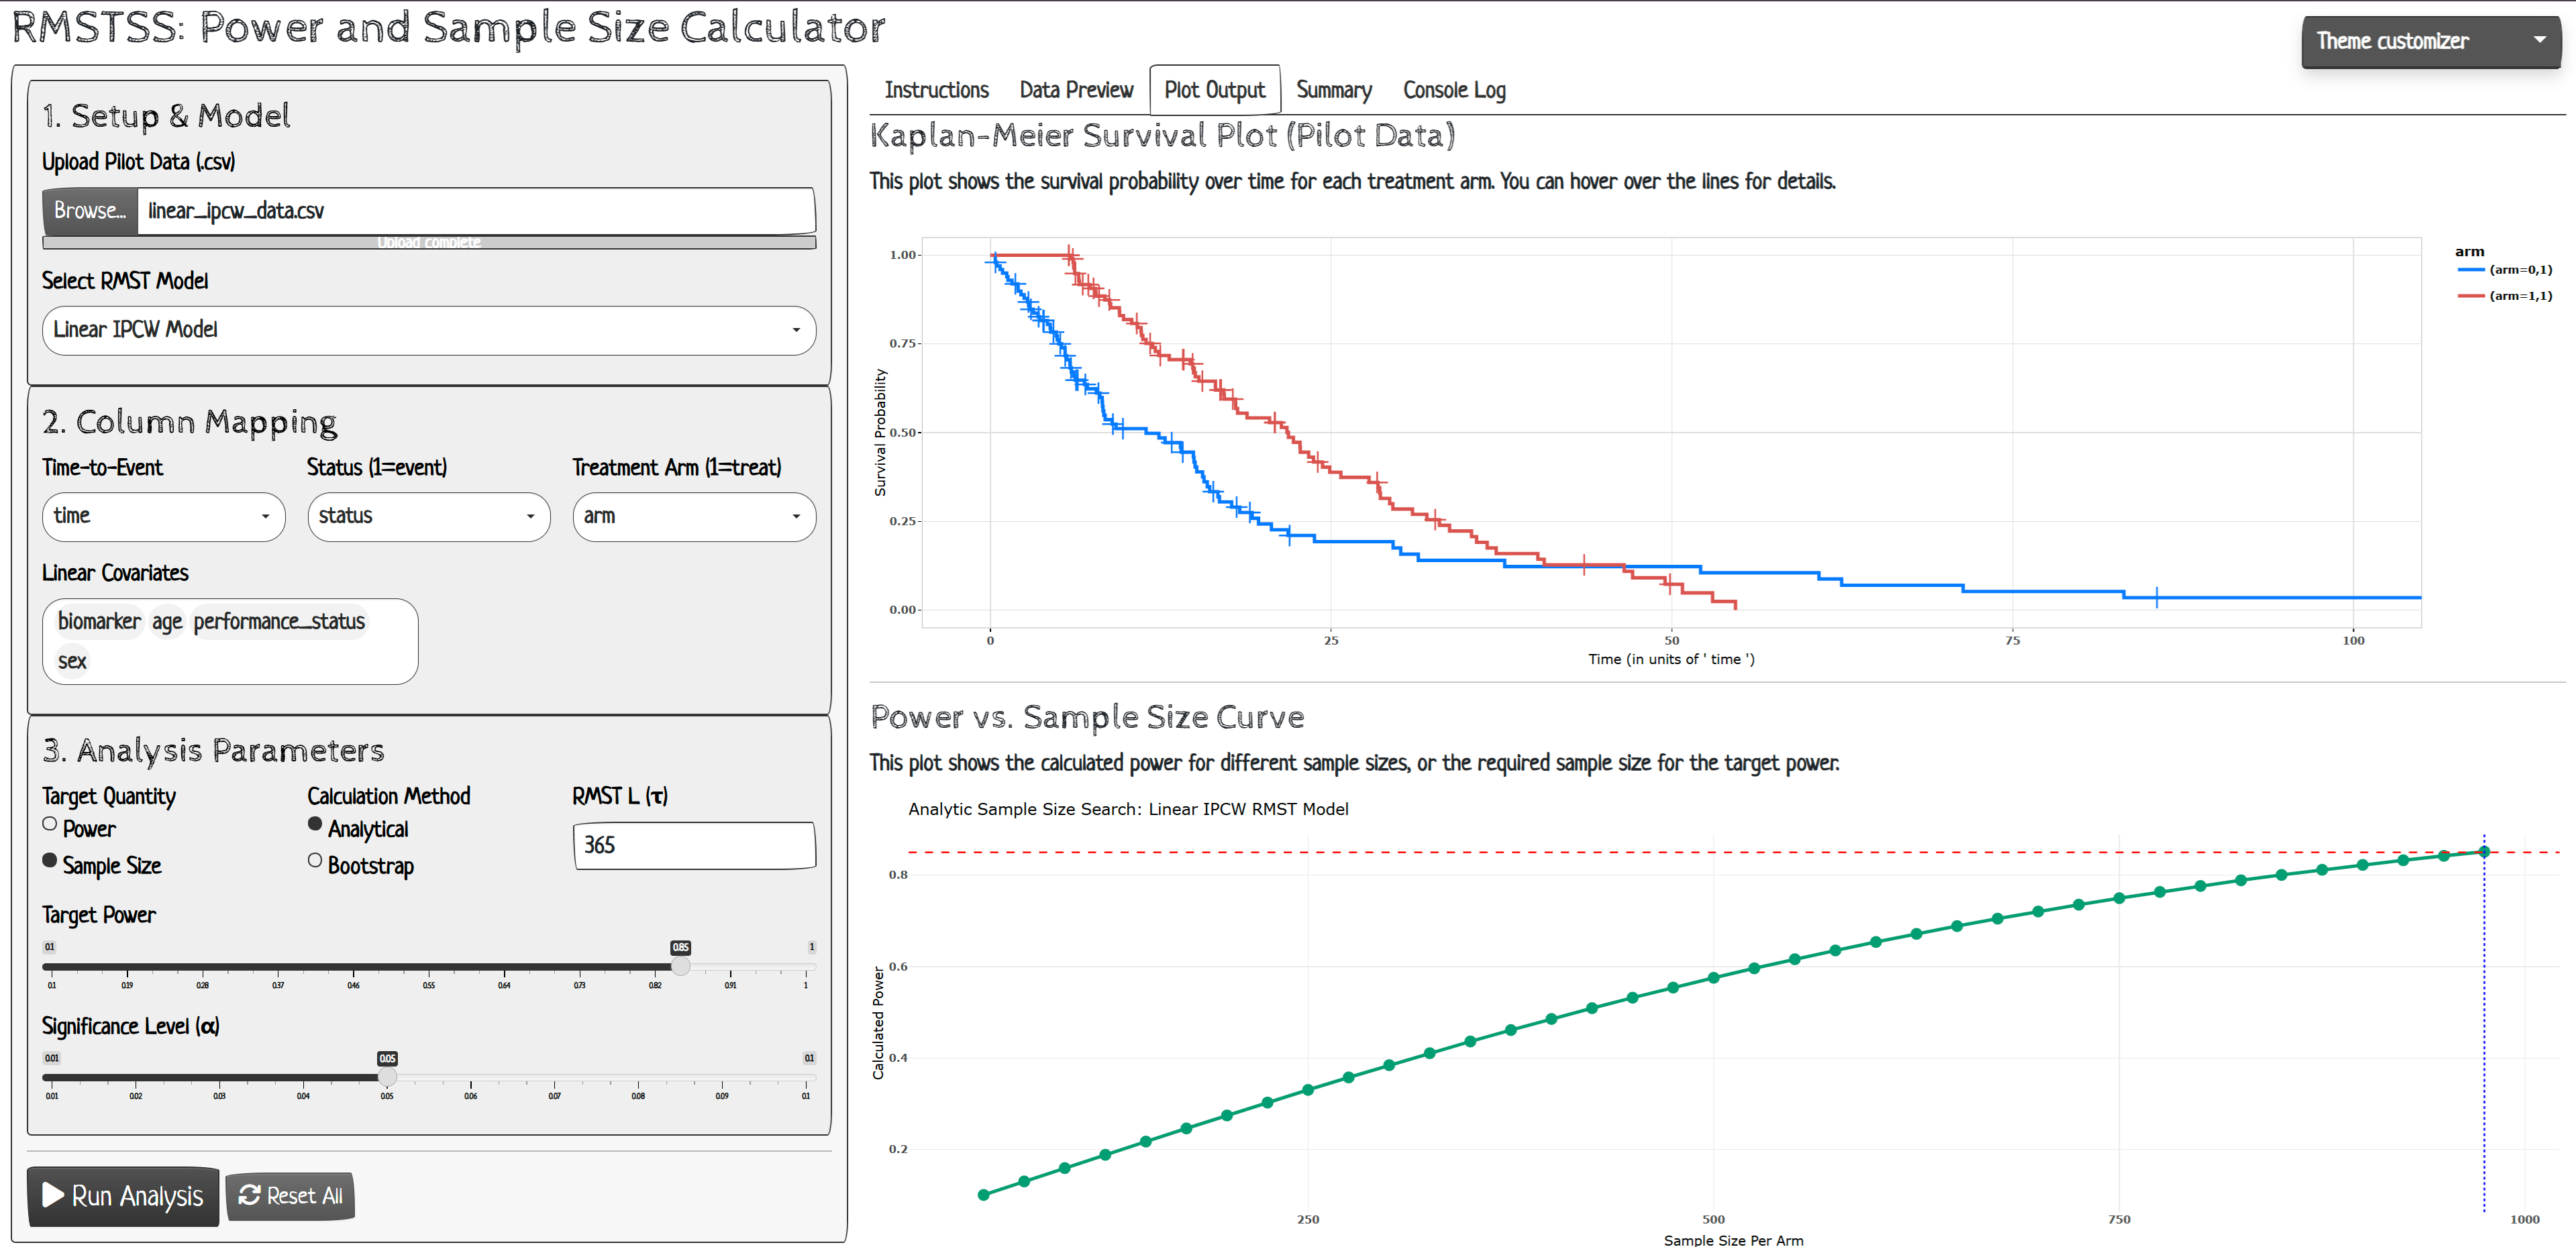
\includegraphics[width=\linewidth]{app-ss.png}
        \vspace{0.25cm}
    \end{center}
    
    \subsection*{\Large How to Use the App}
    \large
    The web app guides you through a simple left-to-right flow:
    \begin{center}
        \Large
        \begin{tabular}{ccccccc}
            \textbf{Upload} & $\boldsymbol{\rightarrow}$ & \textbf{Model} & $\boldsymbol{\rightarrow}$ & \textbf{Target Quantity} & $\boldsymbol{\rightarrow}$ & \textbf{Results!} \\
        \end{tabular}
        
        \vspace{0.2cm}
        \large
        The app allows you to prepare a downloadable report with all the analysis results and console outputs.
    \end{center}

    \subsection*{\Large App Features}
    \begin{itemize} \itemsep=0.25em
        \item \large \textbf{Multiple Models:} Handles standard trials, multi-hospital studies, and more.
        \item \large \textbf{Clear Goals:} Calculate \textbf{Power} or search for the required \textbf{Sample Size}.
        \item \large \textbf{Flexible Methods:} Use a \textbf{Quick Check} (Analytical) or a \textbf{Deep Dive} (Bootstrap).
    \end{itemize}
    
  \subsection*{\huge App Website}
    \begin{center}
        \qrcode[height=5cm]{https://arnab96.shinyapps.io/uthsc-app/}
    \end{center}
\end{posterbox}

\end{minipage}
\hfill % Flexible space between columns
\begin{minipage}[t]{0.32\linewidth} % --- RIGHT COLUMN ---

\begin{posterbox}{The `RMSTSS` R Package}
    \Large
    For statisticians and developers, `RMSTSS` is a powerful R package for use in scripts and analysis pipelines.
    
    \subsection*{\huge Key Functions \& When to Use Them}
    \Large
    The package provides a suite of functions for different trial designs:
    
    \vspace{0.5cm}
    \begin{tabular}{|p{0.35\linewidth}|p{0.55\linewidth}|}
        \hline
        \textbf{\large Function Group} & \textbf{\large Use Case} \\
        \hline
        \texttt{linear.*()} & Standard clinical trials. \\ \hline
        \texttt{additive.*()} & Multi-hospital trials (constant benefit). \\ \hline
        \texttt{MS.*()} & Multi-hospital trials (proportional benefit). \\ \hline
        \texttt{GAM.*()} & For complex, non-linear effects. \\ \hline
        \texttt{DC.*()} & Studies with competing outcomes. \\
        \hline
    \end{tabular}

    \subsection*{\huge Installation and Usage Guide}
    \Large
    Install directly from GitHub:
    \begin{alltt}
remotes::install_github(
"UTHSC-Zhang/RMSTSS-Package"
)
    \end{alltt}
  \Large
  After installing the package the app can be used in local machine using the following code.
      \begin{alltt}
             RMSTSS::run_app()
    \end{alltt}
    
    \subsection*{\huge Project Website}
    \begin{center}
        \qrcode[height=6cm]{https://github.com/UTHSC-Zhang/RMSTSS-Package}
    \end{center}
\end{posterbox}

\end{minipage}

\end{document}